\section{Introduction}
\label{section:hardware:introduction}

\textbf{Benjamin: I think, a more general introduction is needed before one dives into the radiometer equation.}

\subsection{Basics of RFI in radio astronomy} ///ALL
The radiometer equation is fundamental in radio astronomy for determining the sensitivity of a radio telescope. It quantifies the relationship between the observed signal, system temperature, bandwidth, and observation time, offering insight into the minimum detectable signal. The equation is given by:
\[ \Delta S = \frac{2 k_B T_{\text{sys}}}{A_{\text{eff}} \sqrt{2 \Delta f \tau}} \]
where \( \Delta S \) is the minimum detectable flux density in Jansky (1 Jy = $10^{-26}$Wm$^2$Hz$^{-1}$), \( k_B =1.38 \times 10^{-23} \;\text{J} / \text{K}\) is the Boltzmann constant, \( T_{\text{sys}} \) is the system temperature in Kelvin (K), \( A_{\text{eff}} \) is the effective area of the telescope in $m^2$, \( \Delta f \) is the observed bandwidth in Hz, and \( \tau \) is the integration time in seconds (s). This equation underscores the importance of low system temperature, large effective area, broad bandwidth, and long integration time for enhancing the sensitivity and accuracy of astronomical observations.

The sensitivity that can be achieved by modern radio astronomy systems is unrivaled in other radio services and applications. However, this fantastic achievement also comes at a cost. Observations are very susceptible to all kinds of human-made transmissions are other forms of electromagnetic radiation. A cell-phone on the Moon would be among the brightest sources in the sky, at the respective frequencies. 

Astronomers usually refer to these anthropogenic signals as radio frequency interference (RFI), but it has to be pointed out that in legal terms, most of the disturbing features in our data is not considered as RFI by administrations and other spectrum management stakeholders. As the operators of radio transmitters usually have a license, the wanted transmissions, e.g., cell-phone carriers, are perfectly legal. 

In spectrum management, RFI specifically means any kind of unwanted emission, such as near spectral sidelobes, harmonics or intermodulation products, which can leak into the allocated band of another radio service. While the Radiocommunication Sector of the International Telecommunication Union (ITU-R) has acknowledged the requirements of radio astronomy already decades ago, the total amount of spectrum that is allocated to the radio astronomy service is low (\textbf{ADD some numbers}). As a consequence, in addition to measurements in the RAS bands, we are opportunistic -- observing the parts of the spectrum outside of the protected bands wherever and whenever possible at an observatory, as not every active radio service is equally utilised everywhere, 

With more and more digital transmissions, however, the efficiency of spectrum usage has increased significantly in the past years. Therefore, the need increases to deal with humanmade features in our datasets, which can range from flagging affected data samples to making an attempt to fully remove them.

It should be noted that the best form of interference mitigation is still to avoid them in the first place. Radio astronomers have done their part by (mostly) constructing telescopes in fairly remote locations, with as little radio noise background as possible. Often site searches entailed dedicated spectrum monitoring to find the quietest places. Making use of terrain shielding provides additional protection. Furthermore, astronomers participate in national and international spectrum management fora (\textbf{should we name the organisations and fora here?}) to advocate for the protection from new applications in the bands allocated to the RAS.

Only if all these efforts fail -- and this is not rarely the case -- actual RFI mitigation needs to be considered.

\subsection{RFI classification}
\label{subsection:hardware:introduction:classification}

\begin{figure}
    \centering
    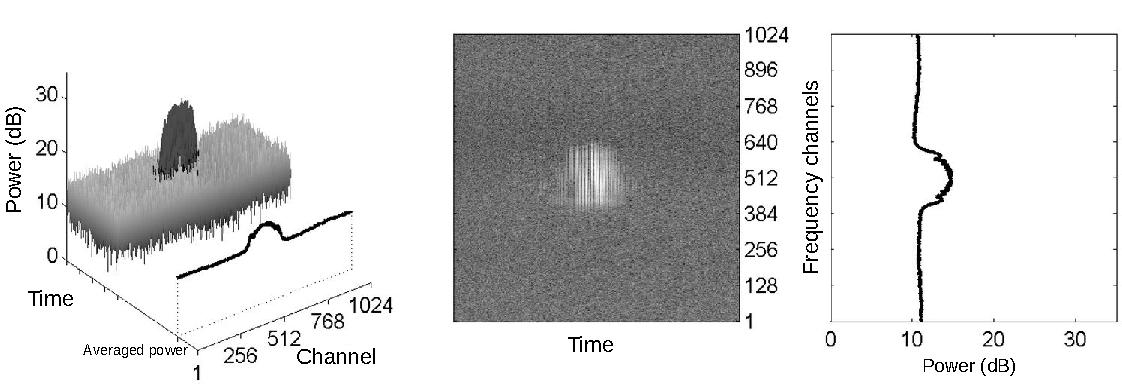
\includegraphics[height=.20\textheight]{figures/radar.pdf}
    \caption{todotodotodo}
    \label{fig:rfi_example_radar}
\end{figure}

\subsection{Levels of RFI}
\label{subsection:hardware:introduction:levels}
A typical radio astronomy receiver chain begins with the feed, which collects incoming radio waves from celestial sources. The feed, often part of a larger antenna system such as a parabolic dish, directs these radio frequency (RF) signals to a low-noise amplifier (LNA). The LNA is crucial as it amplifies the weak astronomical signals while adding minimal noise, ensuring the integrity of the data.

Next, the amplified signal passes through a bandpass filter, which isolates the frequency range of interest. After filtering, the signal is often downconverted from its original high frequency to a lower intermediate frequency (IF) using a mixer and a local oscillator. This downconversion facilitates easier and more accurate signal processing.

The IF signal is then further amplified and may undergo additional filtering before being digitized by an analog-to-digital converter (ADC). The ADC samples the signal at a high rate (typically Mega- to Giga Samples per second (MSps or GSps)), converting it into digital data that can be further processed to extract the astronomical information of interest. With increasing capabilities of modern digital hardware, the downconversion process mentioned above is often not even necessary anymore. Instead, the signal is digitized at the RF frequency. This can be even done close to the receiver box, which minimizes signal degradation when transporting it from the antenna to the computing facility of the observatory.

RFI may occur at various stages in the receiver signal chain, and we distinguish the following levels of impact to the astronomical observation:
\begin{itemize}

\item \emph{Level 0}: at the weakest levels, RFI is undetectable in the telescope signal after a sufficiently long integration time ($\sim$1 hour) and does not impact the science end-product of the observation. The threshold level of such RFI is usually assessed theoretically using an accurate forward modelling effort of the signal processing chain. The level may also be assessed empirically in a controlled experiment involving sensitivity measurements while injecting a controlled RFI signal in the vicinity of the radio telescope. RFI may achieve a weak level when at the telescope site due to long-distance propagation attenuation, side lobe rejection, or signal decorrelation in the context of a phase-tracking radio interferometer.

\item \emph{Level 1}: the RFI reaches the level of an unwanted contribution added to the astronomical information, and impacts the science data. Such RFI requires excision, which consists in detecting the RFI in the signal processing chain, and either subtracting the RFI contribution from the telescope signal, or replacing the impacted data with specific ``flag'' values. The RFI detection may occur in the analog chain, e.g. by monitoring the radio frequency signal power, or in the digital domain by monitoring power excesses in the ADC samples or data sub-integrations for non-time-continuous (i.e. transient) RFI, or in the frequency domain after channelization for band-limited RFI. The RFI excision impacts the sensitivity of the measurement as it effectively either increases $T_{\text{sys}}$ when the excision is applied in the analog domain or reduces $\Delta f$ or $\tau$ when the excision is applied in the digital domain. Additionally, such RFI may prevent the detection of sparse astronomical signals, such as narrow spectral lines in the frequency domain, or transients in the time domain. Detectable RFI may also lead to inaccuracies in telescope data calibration when not accurately identified and accounted for.

\item \emph{Level 2}: stronger RFI will drive elements in the analog signal chain (the LNA in particular) into a non-linear regime, generating harmonics and intermodulation products of one or multiple RFI signals. Similar to \emph{Level 1}, the typical mitigation of RFI at this level requires the detection and excision of the impacted telescope data regions in the time and frequency (TF) domains. The amount of excision is however increased compared to the effective RFI TF footprint, which results in a sensitivity drop in the astronomical observation. A standard mitigation solution of such RFI involves the insertion of power attenuators before the LNA, which in turn also impacts the sensitivity of the telescope even more by increasing the system noise temperature. The RFI threshold of \emph{Level 2} is assessed by accurately measuring the LNA response beyond its linear regime, notably by conducting second- and third-order intercept point (IP2 and IP3) measurements.

It should be pointed out that very broadband receivers can often have strong transmitter signals somewhere in the detected frequency band. Even if these frequencies are not of scientific interest, they can make a complete observation useless. As the transmitters are legally operating, however, some spectrum agencies may not be supportive in such cases and instead ask the observatory to use more robust receivers (e.g. placing stop-band filters in front of the LNA). This in turn will significantly reduce the sensitivity of the observations (as the electronic noise of the filter is amplified, too), creating a real conflict between the scientific needs and the regulatory situation. 

\item \emph{Level 3}: even stronger RFI will lead to analog power levels exceeding the ADC operating range, resulting in signal clipping or saturation in the digital domain. The underlying astronomical information can no longer be recovered at this level because all of the digital TF range is impacted by unpredictable signal artefacts. The maximum RFI power level is directly related to the ADC dynamic range. Typical mitigation solutions at this level involve the insertion of attenuators between the LNA and the ADC, which impacts the measurement sensitivity of the telescope system, or choosing an ADC with an appropriately increased dynamic range.

\item \emph{Level 4}: In extreme cases, a powerful RFI signal entering the telescope receiver can cause excessive heating that is so intense that it melts or burns the receiver components. This situation is exacerbated when the interference is continuous or recurrent, as repeated exposure to high power levels can cumulatively damage the receiver's electronic circuits. This is an undesirable level in which no mitigation can be applied outside of the complete interruption of the telescope operation.
\end{itemize}

It is the aim of RAS spectrum management, to ensure that Level 0 is ensured in all frequency bands allocated on a primary basis to the RAS from inband and out-of-band emissions of active transmitters. In bands not allocated to the RAS, all levels of RFI occur in practice, depending on the environment of the telescope. 

\subsection{Limitations of offline mitigation}
\label{subsection:hardware:introduction:limitations_offline}

\subsection{Motivation for real-time RFI mitigation}
\label{subsection:hardware:introduction: motivations}

Real-time RFI mitigation usually happens in the analog domain or at the highest time resolution (Nyquist rate or a fraction of it), which helps minimize the data corruption in downstream signal processing with minimal loss of astronomical data, thereby improving and enhancing the quality and accuracy of astronomical measurements. Figure 1 illustrates the increase in data loss in a typical radio telescope receiver signal processing chain.
Other benefits from real-time RFI mitigation are as follows:

\begin{enumerate}
\item For time-domain impulsive RFI, the energy spreads across the observing band in the frequency domain, making it impossible to mitigate in the spectral or post-correlation domain.

\item Correlated RFI is best treated in the pre-correlation domain to reduce its ill effects on the astronomical data.

\item RFI is mostly non-random; hence, its early removal helps follow the radiometer equation, which is crucial to achieving the desired sensitivity of the telescope.

\item It helps facilitate adjustments to the telescope signal processing chain in response to a dynamic RFI environment. This adaptability is crucial in maintaining the continuity of observations and ensuring that data collection is optimized even in transient or sporadic RFI.
\end{enumerate}

\begin{figure}
    \centering
    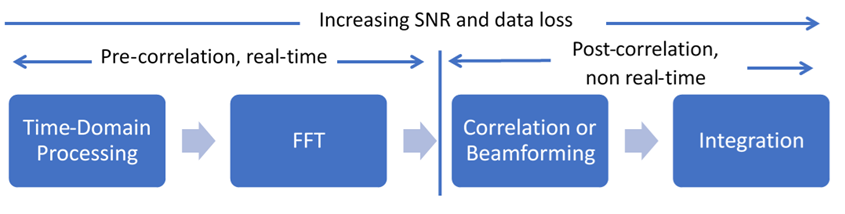
\includegraphics[scale=0.8]{Hardware Excision Techniques/figures/rt.jpg}
    \caption{SNR versus data loss in a typical telescope receiver system}
    \label{fig:real-time-rfi}
\end{figure}


Additionally, real-time RFI mitigation contributes to the protection and longevity of sensitive receiver components by promptly handling high-power interfering signals and reducing the risk of thermal damage and long-term degradation of electronic components.
While real-time detection and excision of RFI is beneficial in radio astronomy it comes with challenges. The main challenge is the cost and power consumption. Even though RFI has become a significant threat to radio astronomy for several decades, few signal chains of radio telescopes have been designed considering the real-time excision of RFI. Hence, the real-time RFI excision methods deployed in existing radio telescopes are implemented using the remaining resources after implementing the key signal processing modules and operated with limited power. Regarding quality, one of the main checks that needs to be made is the flagging duration and accuracy of flagging.  It should be ensured that the excision is optimal i.e. there is no over-excising of the data which can result in the loss of precious observational data or under-excising which leads to RFI remnants in the data.


An example of a real-time RFI mitigation released and operational for the uGMRT including the possibility of extending it to contemporary and upcoming telescopes is provided in \cite{buch2023real}.










%\subsubsection{Thushara}
%Real-time RFI excision enables radio astronomers to salvage observations taken in a contaminated segment of the observation band, either when the RFI source is not transmitting or when the RFI strength is attenuated to a level below the ITU recommended threshold\citep{ITU_protection_2003}. For example, consider the interference caused by strong radio pulses emitted by the Distance Measuring Equipment (DME) of an aircraft \cite{wiki_dme_2024}, which are being picked up by the antennas of radio telescopes. The DME pulses transmit in bands within 960-1215 MHz at a power level of 1 kW. Each DME pulse is 3.5 µs wide and repeats every 12 µs for a second or so in a single burst. Normally, the DME pulses are detected by the sidelobes of the antennas of a radio telescope. These pulses can be fairly easy to detect at the front of the signal chain of the radio telescope, which is operating at a wider bandwidth. Once detected, the contaminated data can be flagged in real-time to prevent further contamination of the accumulation. Also, RFI detection carried out along the various stages of the signal chain of a radio telescope allows radio astronomers to maintain the linearity of the signal chain with proper scaling while achieving the maximum possible dynamic range for a given set of computational resources.

%While real-time detection and excision of RFI is beneficial in radio astronomy it comes with challenges. The main challenge is the cost and power consumption. Even though RFI has become a significant threat to radio astronomy for several decades or so few signal chains of radio telescopes have designed considering the real-time excision of RFI. Hence, the real-time RFI excision methods deployed in existing radio telescopes are implemented using the remaining resources after implementing the key signal processing modules and operated with limited power. In terms of quality, one of the main drawbacks of real-time RFI excision is the uncertainty of the flagging duration.  This leads to either over-excising the data resulting in the loss of precious observations or under-excising which leads to RFI remnants causing artifacts in the observations. 

%\subsubsection{Kaushal - Motivation for Real-time RFI Mitigation}

%Real-time RFI mitigation usually happens at the highest time resolution (Nyquist rate) which helps prevent data corruption in downstream signal processing with minimal loss of astronomical data. Other benefits from real-time RFI mitigation are as follows:

%1. For time-domain impulsive RFI, the energy 
%spreads across the observing band upon Fourier
%transformation, making it difficult to detect and
%mitigate in the post-processing operation.

%2. Mitigation in the pre-correlation domain helps
%reduce the ill effects of correlated RFI.

%3. RFI is mostly non-random and hence its early removal helps in following the radiometer equation which is crucial to achieve the desired sensitivity of the telescope.

%\subsubsection{Greg}
%Real-time RFI mitigation is a critical capability of modern radio telescopes that facilitates adjustments to the telescope signal processing chain in response to a dynamic RFI environment. This adaptability is crucial in maintaining the continuity of observations and ensuring that data collection is optimized despite the presence of transient or sporadic RFI. It also enhances the quality and accuracy of the collected astronomical information by identifying, attenuating, or excising corrupted data at the highest data rates before any data compression, and preventing the saturation of the vulnerable receiver components (e.g. LNA or ADC).

%Mitigating RFI in real-time also helps minimizing the downstream computational load and storage requirements by processing the RFI contribution at the point of data acquisition rather than further down the signal chain. This strategy alleviates the need for storing intermediate data products, which can be unbearbel with the increase of telescope bandwidths and array sizes.

%Additionally, real-time RFI mitigation contributes to the protection and longevity of sensitive receiver components by promptly handling high-power interfering signals and reducing the risk of thermal damage and long-term degradation of electronic components.

